In diesem Versuch wird die Relaxationslänge schneller Neutronen und die Diffusionslänge thermischer Neutronen in Wasser gemessen.

\section{Ausbreitung schneller Neutronen in Materie}

Neutronen sind ungeladene Teilchen. Sie wechselwirken hauptsächlich durch die folgenden Prozesse mit Materie:
\begin{itemize}
 \item Elastische Streuung: Dabei ist die Energie der Stoßpartner erhalten. Da die Kerne vor dem Stoß in Ruhe sind, verliert das Neutron dabei Energie. Der Energieverlust ist am größten, wenn die Massen der Stoßpartner gleich sind. Daher ist der Energieverlust der Neutronen für die Streuung an Protonen besonders groß.
	Der Wirkungsquerschnitt für die elastische Streuung ist für niederenergetische (thermische) Neutronen am größten (s. Abb. \ref{fig:np}).
 \item Absorption: Hierbei wird das Neutron vom Kern aufgenommen. Dabei kann eine Kernreaktion induziert werden.
 \item Inelastische Streuung: Hier wird dem Kern Anregungsenergie übertragen. Daher ist der Energieverlust der Neutronen größer als bei der elastischen Streuung. Die Wirkungsquerschnitte für solche Reaktionen sind jedoch geringer.
\end{itemize}

Der Fluss der Neutronen im Abstand $r$ zu einer punktförmigen Quelle monoenergetischer Neutronen ist dann gegeben durch \cite{BB}
\begin{equation}
 \phi(r) = \frac{Q}{4\pi r^{2}}\exp\left( -\Sigma_{t}r\right),
\end{equation}
wobei $Q$ die Quellstärke und $\Sigma_{t}$ den totalen linearen Absorptionskoeffizienten bezeichnet. Der Abfall proportional zu $\frac{1}{r^{2}}$ ergibt sich aus der Erhaltung der Gesamtanzahl der Neutronen, die durch eine Kugeloberfläche fliessen.
Der Faktor $\exp\left( -\Sigma_{t}r\right)$ entspricht den absorbierten Neutronen. Die Relaxationslänge wird definiert als
\begin{equation}
 \lambda = \frac{1}{\Sigma_{t}}.
\end{equation}
Diese Verteilung gilt nur für sogenannte Primärneutronen, die noch keine Reaktion mit der Materie durchgeführt haben.

\section{Ausbreitung thermischer Neutronen in Materie}

Wechselwirken Neutronen genügend lange mit der Materie, so geben sie ihre überschüssige Energie an diese ab. Sie befinden sich dann im thermischen Gleichgewicht mit der Materie und ihre Geschwindigkeitsverteilung ist die Maxwellsche Geschwindigkeitsverteilung.
Ihre mittlere Energie bei der Temperatur $T$ ist dann gegeben durch
\begin{equation}
 \overline{E} = k_{\textrm{B}}T.
\end{equation}

Unter der Vorraussetzung eines energieunabhängigen Streuquerschnittes $\Sigma_{s}$ und schwacher Absorption $\Sigma_{a}<<\Sigma_{s}$ (auch energieunabhängig) gehorchen die thermischen Neutronen der Diffusionsgleichung
\begin{equation}
 \mathcal{4} \phi - \frac{1}{L^{2}}\phi + \frac{S(r)}{D} = 0,
\end{equation}
mit der Diffusionskonstanten $D=\frac{1}{3\Sigma_{a}}$, der Diffusionslänge $L=\sqrt{\frac{D}{\Sigma_{s}}}$ und der Emission der Quelle $S(r)$. Mit der Randbedingung, dass $\phi$ im Unendlichen verschwindet ergibt sich
\begin{equation}
 \phi(r) = \frac{Q}{4\pi D r}\exp\left( -\frac{r}{L}\right).
\end{equation}

\begin{figure}[tb]
  \centering
  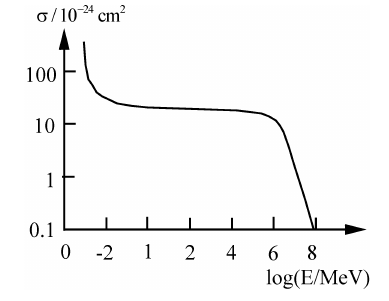
\includegraphics[scale=1.0]{./fig/np_streuung.png}
  \caption{Wirkungsquerschnitt für Neutron-Proton-Streuung \cite{BB}}
  \label{fig:np}
\end{figure}

\section{Die Neutronenquelle}

Im Versuch wird eine Am-Be-Neutronenquelle verwendet. Dabei dient $^{241}$Am als $\alpha$-Quelle. Die $\alpha$-Teilchen treffen auf die $^{9}$Be-Kerne und regen die folgende Reaktion an
\begin{equation}
 ^{9}\textrm{Be} + \alpha  \longrightarrow \textrm{n} + ^{12}\textrm{C} + Q.
\end{equation}
Dabei ist $Q=\SI{5,7}{\mega\electronvolt}$ die bei der Reaktion freiwerdende Energie, die hauptsächlich auf das Neutron übergeht. Da die Neutronen unter beliebigen Winkeln in Bezug auf das einfallende $\alpha$-Teilchen emittiert werden, ist das Spektrum der Neutronenquelle kontinuierlich.
Die maximal mögliche Neutronenenergie ist gegeben durch
\begin{equation}
 E_{\textrm{max}} = Q + E_{\alpha} - E_{\textrm{r}} = \SI{11,19}{\mega\electronvolt}.
\end{equation}
Hier bezeichnet $E_{\alpha}$ die Energie des $\alpha$-Teilchens und $E_{\textrm{r}}$ die Rückstoßenergie, die vom $^{12}$C-Kern aufgenommen wird.

\section{Versuchsdurchführung}

\subsection{Bestimmung der Relaxationslänge}

Um die Relaxationslänge $\lambda$ schneller Neutronen in Wasser zu messen, wird die Anzahl der Neutronen pro Zeiteinheit in Abhängigkeit des Abstandes von der Quelle gemessen. Es wird im Bereich $14$ bis $\SI{19}{\centi\metre}$ gemessen.
Da der Neutronenfluss proportional zur Anzahl der Neutronen ist, und da die anderen relevanten Größen (Zeitintervall und Detektorfläche) nicht variiert werden, kann daraus die Relaxationslänge bestimmt werden. Durch Logarithmieren des Flussgesetzes ergibt sich
\begin{equation}
 \ln\left(Nr^{2}\right) = -\frac{r}{\lambda} + C,
\end{equation}
mit der Anzahl der Neutronen $N$, der Distanz zur Quelle $r$ und einer Konstanten $C$. Durch eine lineare Regression kann nun $\lambda$ bestimmt werden.

Die Vorraussetzungen, damit dieses Flussgesetz gilt, sind jedoch im Experiment nicht erfüllt. Das $^{10}$B-Zählrohr kann nur Neutronen bis zu einer Energie von ca. $\SI{100}{\kilo\electronvolt}$ detektieren. Somit werden gerade die schnellen Neutronen nicht gemessen. Dennoch folgt die folgt die Verteilung der Neutronen im Experiment dem obigen Zusammenhang.
Der Grund dafür ist, dass die langsamen Neutronen sehr stark an den Protonen des Wassers gestreut werden. Dabei verlieren sie einen Großteil ihrer Energie. Daher entfernen sie sich nur bis ca. $\SI{3}{\centi\metre}$ von der Quelle. 
Der gemessene Fluss verhält sich daher für Abstände $>>\SI{3}{\centi\metre}$ wie der Fluss schneller Neutronen.

\subsection{Bestimmung der Diffusionslänge}

Um die Diffusionslänge $L$ thermischer Neutronen in Wasser zu messen, kann nicht auf analoge Weise zum vorherigen Versuch vorgegangen werden, da es keine punktförmige Quelle thermischer Neutronen gibt.
Stattdessen wird die sogenannte Cd-Differenzmethode verwendet. Dazu wird die Quelle mit Hilfe einer dünnen Cadmium-Kugelschale abgeschirmt. Der Absorptionsquerschnitt für Neutronen in Cadmium (s. Abb. \ref{fig:cd}) ist für thermische Neutronen deutlich größer als in den anderen Energiebereichen. Daher durchqueren nur schnelle Neutronen die Kugelschale.
Durch Differenzbildung mit dem gesamten Fluss erhält man den Fluss einer thermischen Neutronenquelle. Die Diffusionslänge kann nun durch eine lineare Regression der Form
\begin{equation}
 \ln\left(N_{d}r\right) = -\frac{r}{L} + C,
\end{equation}
mit der Differenz der Neutronenzahlen $N_{d}$, bestimmt werden.

\begin{figure}[h]
  \centering
  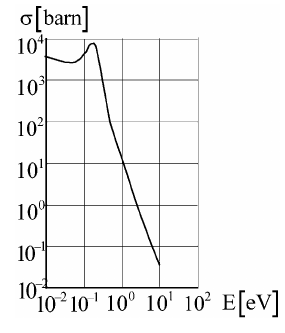
\includegraphics[scale=1.0]{./fig/cd_wirkungsquerschnitt.png}
  \caption{Absorptionsquerschnitt für Neutronen in Cadmium \cite{BB}}
  \label{fig:cd}
\end{figure}